\documentclass[useAMS,usenatbib]{mn2e}
\usepackage{graphicx}
\usepackage{amssymb}
\usepackage{natbib}
\bibliographystyle{mn2e}
\pdfminorversion=5   % recommended by MNRAS web page


%%% Journal abbreviations.
\def\apj{ApJ}                 % Astrophysical Journal
\def\apjl{ApJL}               % Astrophysical Journal, Letters
\def\apjs{ApJS}               % Astrophysical Journal, Supplement
\def\mnras{MNRAS}             % Monthly Notices of the RAS
\def\aap{A\&A}                % Astronomy and Astrophysics
\def\aaps{A\&AS}              % Astronomy and Astrophysics, Supplement
\def\aj{AJ}                   % Astronomical Journal
\def\physrep{Phys.~Rep.}      % Physics Reports
\def\nat{Nature}              % Nature
\def\araa{ARA\&A}             % Annual Review of Astronomy and Astrophysics
\def\planss{planss}           % Planetary and Space Science
\def\ssr{SSR}                 % Space Science Reviews
\def\sovast{Sov.~Astron.}     % Soviet Astronomy
\def\canjphys{Can. J. Phys.}  % Canadian Journal of physics
\def\nar{New~Astron.}

 
\newcommand{\msun}{{M$_\odot$}}

\topmargin -1cm


\title{Cooling Clouds by Varying Metallicities: Origin of Globular Cluster Bimodality}

\author[R. Fernandez et al.]{Ricardo Fernandez$^{1}$ and Greg L. Bryan$^{1}$\\
$^{1}$Department of Astronomy, Columbia University, 550 West 120th Street, New York, NY 10027, USA}

\begin{document}

\date{}

%\pagerange{\pageref{firstpage}--\pageref{lastpage}} \pubyear{2013}

\maketitle

%\label{firstpage}

\begin{abstract}
Globular Clusters
\end{abstract}

\begin{keywords}
globular clusters - methods:numerical
\end{keywords}

%% ----------------------------------------------------------------
%
\section{Introduction}

Globular clusters (GCs), with typical masses of $10^5$-$10^6$ \msun\ are particularly interesting relics of star formation for a number of reasons: (1) the are very concentrated, with half-mass radii of a few parsecs, indicating that star formation occurred in a particularly dense environment; (2) the stars in a given GC generally have a very narrow spread in ages and metallicity, implying a single stellar population (although recent results have revealed a more nuanced situation here, as we will discuss briefly later), and (3) the metallicity distribution of GCs in external galaxies is generally bimodal (or at least very different from the metallicity distribution of stars in the galaxy as a whole), with a large number of low-metallicity GCs.  Reviews of their properties include Brodie \& Strader (2006), Renzini (2008, 2013), and see also Protegies et al (2010).

This bimodal, or possibly skewed metallicity distribution (e.g. Strader et al. 2003, Peng et. al 2006) is sometimes interpreted as indicating that there are two formation modes: one that produced low-metallicity, old systems and a second for the generally younger, higher-metallicity component.  For instance, Ashman \& Zepf (1992) suggested that metal-rich GCs are formed in gas rich mergers and metal-poor GCs are donated by progenitor spirals.  However, their work did not incorporate a cosmological model, and their predictions of the number and color distribution of GCs in massive Es galaxies were not consistent, as pointed out by Forbes, Brodie \& Grillmair (1997).  Other models explored reionization for setting the bimodality (e.g., Santos 2003; Harris \& Pudritz 1994).

Beasley et al. (2002) augmented this picture by incorporating a semi-analytical model of combined galaxy and GC formation in a cosmological context. In that work, each mode of GC formation was assigned a fixed efficiency relative to the field stars. However, to match observed values, the formation of metal-poor GCs had to be artificially truncated after $z = 5$. Recently, investigations have explored more empirical, hierarchical galaxy formation models in a cosmological setting.   Muratov \& Gnedin (2010) have modeled the formation of GCs using the assembly history from cosmological simulations combined with observed scaling relations. In their model bimodality naturally arises from the rate of galaxy mergers. Early mergers preferentially produce metal-poor GCs and a few late massive mergers can produce a significant number of metal-rich GCs.  However their model produces metal-rich GCs that are too young, which is at odds with observation that some of metal-rich GCs are old as metal-poor GCs. In addition, their model is again semi-analytic and doesn't explicit deal with how star formation proceeds in low-metallicity, high-density gas.

Essentially none of the models discussed above attempt to model the detailed structure of star formation within globular clusters.  In particular, it is not clear how to get a large amount of gas ($10^6$ \msun) into a very small region without star formation occurring during the collapse, which would result in a wide spatial distribution of stars and perhaps even prevent the collapse.  

As an aside, we note that, quite recently, observations have demonstrated that globular clusters are not a single stellar population, but may be composed of multiple generations showing enhanced He and specific abundance changes, particularly those associated with proton-capture processes (e.g., Norris et al 1981; Kraft 1994; Gratton et al. 2001; Carretta et al. 2009).  In addition, photometric data shows a splitting of the man sequence in many GCs (e.g., Piotto 2009; Anderson et al. 2009; Milone et al. 2010).  This has been challenging to explain because, with a few possible exceptions, the Fe abundence distribution is generally very narrow (consistent with observational errors), indicating that supernova self-enrichment plays no role.  A wide range of models have been proposed to explain these abundance irregularities, beginning with the possibility that AGB stars in the 4-8 \msun\ mass range can produce the necessary elements through hot bottom burning (e.g., D'Ercole et al 2010; Ventura et al. 2013).  Other ideas include the existence of Fast Rotating Massive Stars (FRMS; Krause et. al 2013), supermassive stars (Denissenkov \& Hartwick 2014; Denissenkov et. al 2015), and massive interacting binaries (e.g. Mink 2009; Bastian et al. 2013).  All of these solutions are problematic for a number of reasons (e.g. Renzini et al. 2015; Bastian et al. 2015), including the mass budget required to generate the observed number of second generation stars.  However, in this work, we will not explicitly explore this second generation, instead focusing on the problem of understanding star formation in low-metallicity gas.


%% ----------------------------------------------------------------
%
\section{Basic Idea}
\label{sec:basic}

In this paper, we explore a simple idea: can the cooling properties of low-metallicity gas clouds themselves influence how star formation proceeds?  High-metallicity (by which we mean approximately solar metallicity, or even lower -- we will address this point more precisely below) gas cools rapidly, typically on a timescale shorter than the dynamical time, meaning that present day large gas clouds, with masses in the GC range, are typically ``cold", with temperatures well below their virial temperatures and so rapid fragmentation is inevitable.  This generally means that high-metallicity giant molecular clouds will rapidly produce stars before they are completely collapsed and feedback from those stars will result in a low star formation efficiency (REF).  However, for a low enough metallicity, the gas may cool slowly so that the cloud will collapse coherently, not fragmenting until the central gas density is very high.  These high densities promote rapid star formation resulting in high efficiency.  In this way, paradoxically, inefficient cooling may result in more efficiency star formation.

To futher investigate this simple idea we have created one zone models of a cooling parcel of gas. In 
this scenario, the parameter space consists of density, temperature, and metallicity. Once the parameters
are chosen the evolutionary timescales are computed: the quantity of interest is the ratio of the absolute value of cooling
time to dynamical time $|t_{cool}|/t_{dyn}$. In our simple one zone model, cooling is computed using the
publicily available \textsc{grackle} chemistry library; details of implementation and functionality can be found
in \cite{Bryan2013}.
\begin{figure}
\begin{center}
\mbox{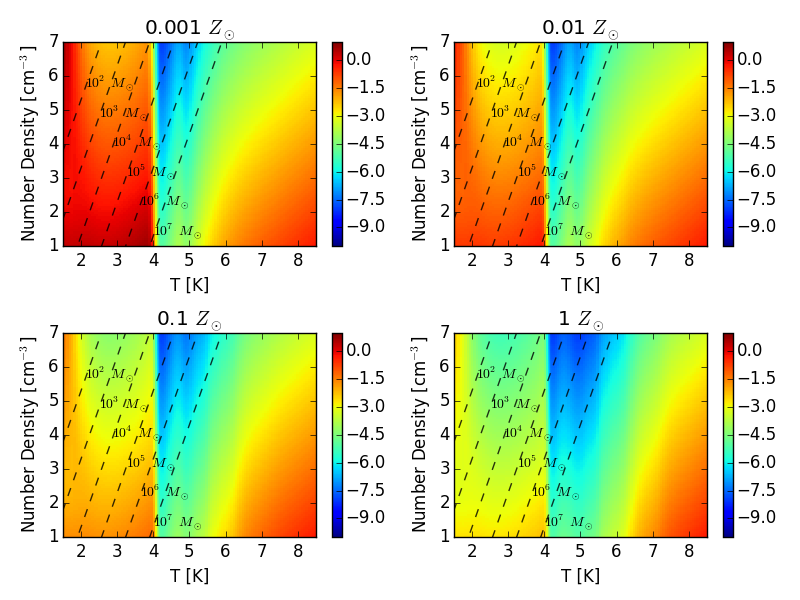
\includegraphics[width=8.5cm]{Images/cooling_to_freefall_no_background}}
\end{center}
\caption{\label{fig:cooling_to_freefall} The ratio of cooling time to dynamical time for gas with a range of density, temperature and metallicity values, as labelled.}
\end{figure}

Figure~\ref{fig:cooling_to_freefall} is a panel showing the ratio of log$(|t_{cool}|/t_{dyn})$
for metallicity values $Z/Z_{\odot}=10^{-3},10^{-2},10^{-1},1$.  To begin, we focus on the lowest metallicity 
(upper-left) panel of Fig~\ref{fig:cooling_to_freefall} -- we see that there
are two regions where cooling and dynamical time are comparable (shaded red). The first is in the temperature range $10^1-10^4$K (the sharp cutoff at $10^4$K is due to efficient cooling from HI line emission), and the second is in the bottom right
corner. It is the former region in which we are most interested because this area is where we expect to find gas clouds with
values conducive for globular cluster formation. Over each heat map, we plot lines of density and temperature corresponding to constant Bonner-Ebert mass (see Section~\ref{sec:numerical} for details on how this is computed). It is clear from the plot that,
for gas clouds with masses typical of globular clusters, there are 
values in the region where cooling is relatively inefficient, allowing the gas to collapse coherently before it can cool and fragment. Further, as the metallicity
increases this region becomes less pronounced and the gas becomes more efficient in cooling, which will allow the gas to cool and fragment before global collapse sets in.

\begin{figure}
\begin{center}
\mbox{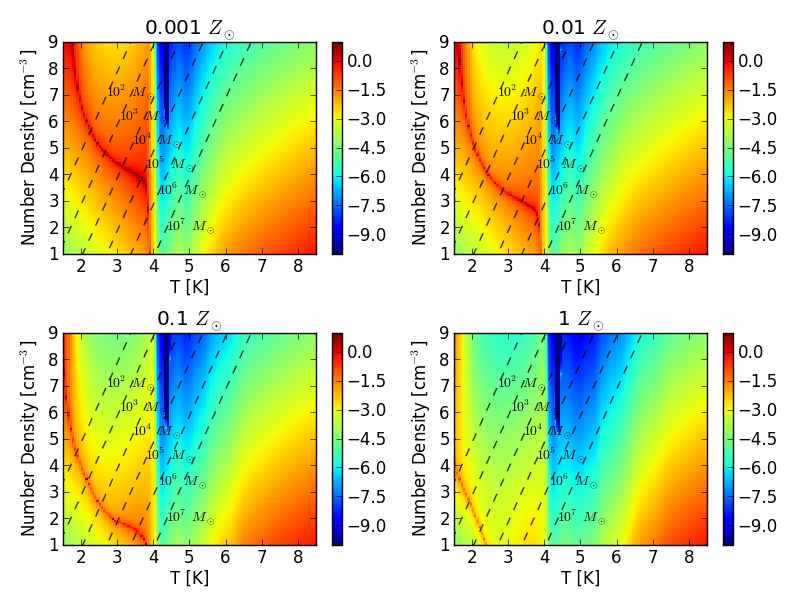
\includegraphics[width=8.5cm]{Images/cooling_to_freefall}}
\end{center}
\caption{\label{fig:cooling_to_freefall_background} The ratio of cooling time to dynamical time for gas with a range of density, temperature and metallicity values, as labelled.  This plot is similar to Figure~\ref{fig:cooling_to_freefall}, except that we include a radiative heating source as specified in \citet{Haardt2012}, at $z=$0.}
\end{figure}

This is all computed in the absence of any radiative background.  In Figure~\ref{fig:cooling_to_freefall_background}, 
the one zone models are recalculated as previous except allowing for radiative heating.   Although the radiative background
is uncertain, we adopt the radiative background from \citet{Haardt2012} at $z=$0 
in order to show the kind of effect we expect.  This does not change the high gas cooling rate, but it does affect the lower-temperature gas cooling time.   In particular, we see that an equilibrium curve is present where
heating and cooling are balanced. We no longer have the extended region where cooling and dynamical time scales are 
comparable but now are concentrated along the equilibrium curve. Furthermore, it should be expected that gas will
naturally seek the equilibrium curve values. Therefore, for values above and below the curve there should be a migration
to high density low temperature for values above and low density high temperature for values below.  Moreover, when the
the metallicity increase the equilibrium curve shifts downward, decreasing the possibility of having globular cluster
like conditions.

This is all determine by computing cooling and dynamical times for gas with a characteristic density and temperature, demonstrating that the idea of inefficient cooling may be appropriate for low-metallicity gas (or gas with a somewhat higher metallicity but stronger radiative background).   We now turn to space- and time-dependent numerical simulations to explore this idea further.  Ideally, we would carry out cosmological simulations that included the full range of dynamical processes relevant for star formation at high-redshift with low (but non-zero) metallicity.  However, this is computational intractable, and therefore we instead investigate a simple, idealized set up.  We expect that gas cloud collisions during mergers at high-redshift will result in the accumulation of gas in relatively dense knows.  These clouds will rapidly cool to temperatures around $10^4$ K.  Therefore, we set up turbulently perturbed Bonner-Ebbert spheres with masses typical of globular clusters, and densities/metallicities motivated by Figure~\ref{fig:cooling_to_freefall}.   In future work, we will explore more complicated dynamics, such as colliding flows; however, here we explore perhaps the most simple possible test of this idea.



%% ----------------------------------------------------------------
%
\section{Numerical Models}
\label{sec:numerical}
\subsection{Numerical Method}

The simulations in this paper were performed with the publicly available Eulerian three-dimensional
hydrodynamical adaptive mesh refinement Enzo code \citep{Bryan2013}. The domain
box size of the simulation was 150 pc on a side with a top level root grid resolution of $128^3$, and
a maximum refinement level of 3, for a cell size of 0.125 pc.  Cell refinement was dictated 
by the gas mass such that a cell was refined whenever the its mass became larger than 0.1 M$_\odot$.
In addition, we refined based on the Jeans length such that it was
always refined by at least 4 cells.

Our simulations included self gravity and radiative cooling using the
Grackle library; details described in \cite{Bryan2013}. The metal cooling (and
heating) rates are computed using a non-equilibrium model for H, H$^+$, He, He$^+$, He$^++$ and e$^-$
and a table computed from Cloudy for metal-line cooling (and heating), as described in Smith et al. (????).
When a radiative background is included, we use \cite{Haardt2012} at $z=$0

\subsection{Initial Conditions}
Our initial conditions consist of a cloud in pressure equilibrium with an
constant ambient density and temperature background. The internal structure of the
cloud is modeled by a Bonner-Ebert sphere \cite{Bonnor1956}: a self-gravitating
isothermal gas sphere in hydrostatic equilibrium embedded in a pressurized  
medium. To fully describe a Bonner-Ebert sphere, a mass $M_{BE}$, temperature
$T_{BE}$, and an external pressure $P_{ext}$ must be chosen. Following our
assumptions outlined in Section~\ref{sec:basic}, we chose
$M_{BE}=10^6$ \msun, $T_{BE}=6000$ K, and $P_{ext}=1.8\times10^5\times k_B$, 
where $k_B$ is the Boltzmann constant. This corresponds to a cloud on the point of
gravitational collapse within nearly comparable cooling and collapse times,
depending the chosen metallicity (which we will vary).

In addition, we add turbulence to the cloud following a power spectrum of
$v_k^2 \propto k^{-4}$ for the velocity field.  We include only mode between
$k_{\rm min}=$ 9 and $k_{\rm max} =$ 19 {\bf (units?)} such that the input modes are well resolved
and have wavelengths smaller than the cloud radius.  We set the turbulent velocities
such that rms velocity of the gas is XXX km/s. Figure~\ref{fig:initial_setup} shows 
a slice through the center of the cloud with four panels providing
the initial number density, temperature, velocity magnitude and pressure.  We use
this initial conditions for essentially all of the runs analyzed in this paper.

\begin{figure}
\begin{center}
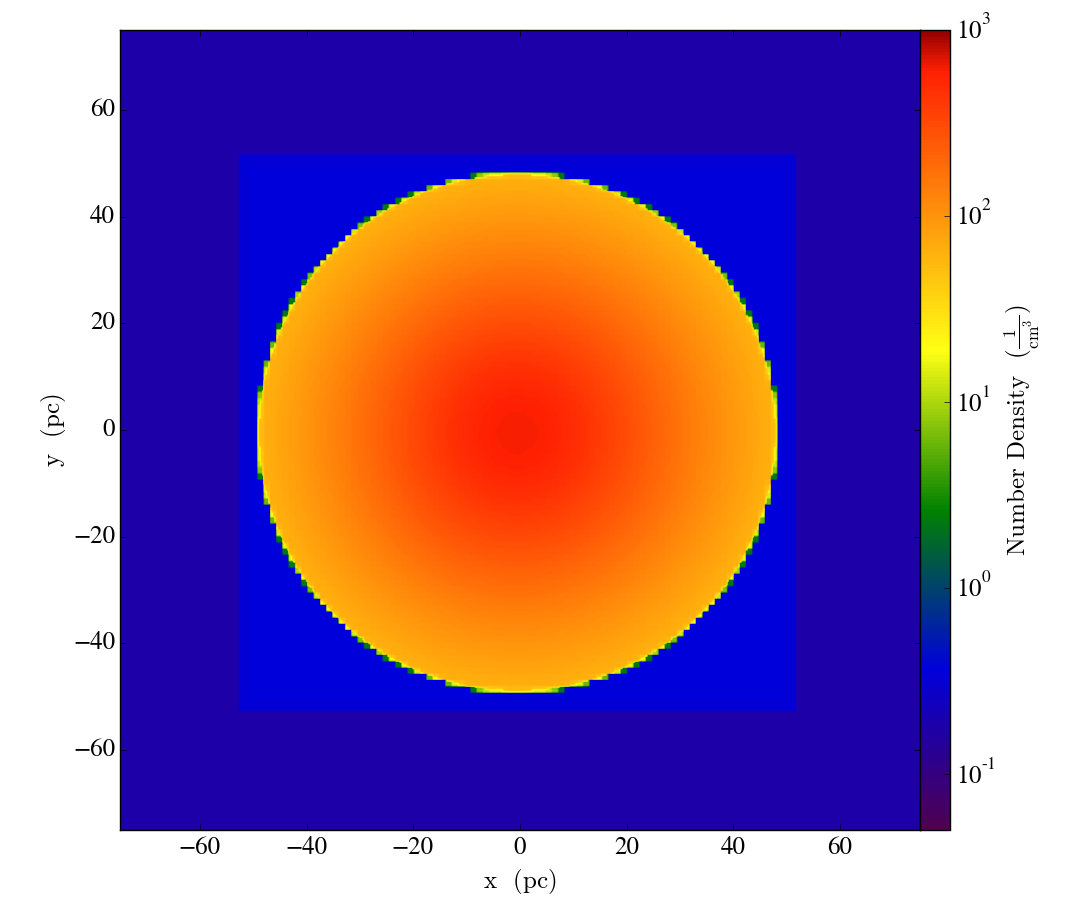
\includegraphics[width=6cm]{Images/Initial_number_density}
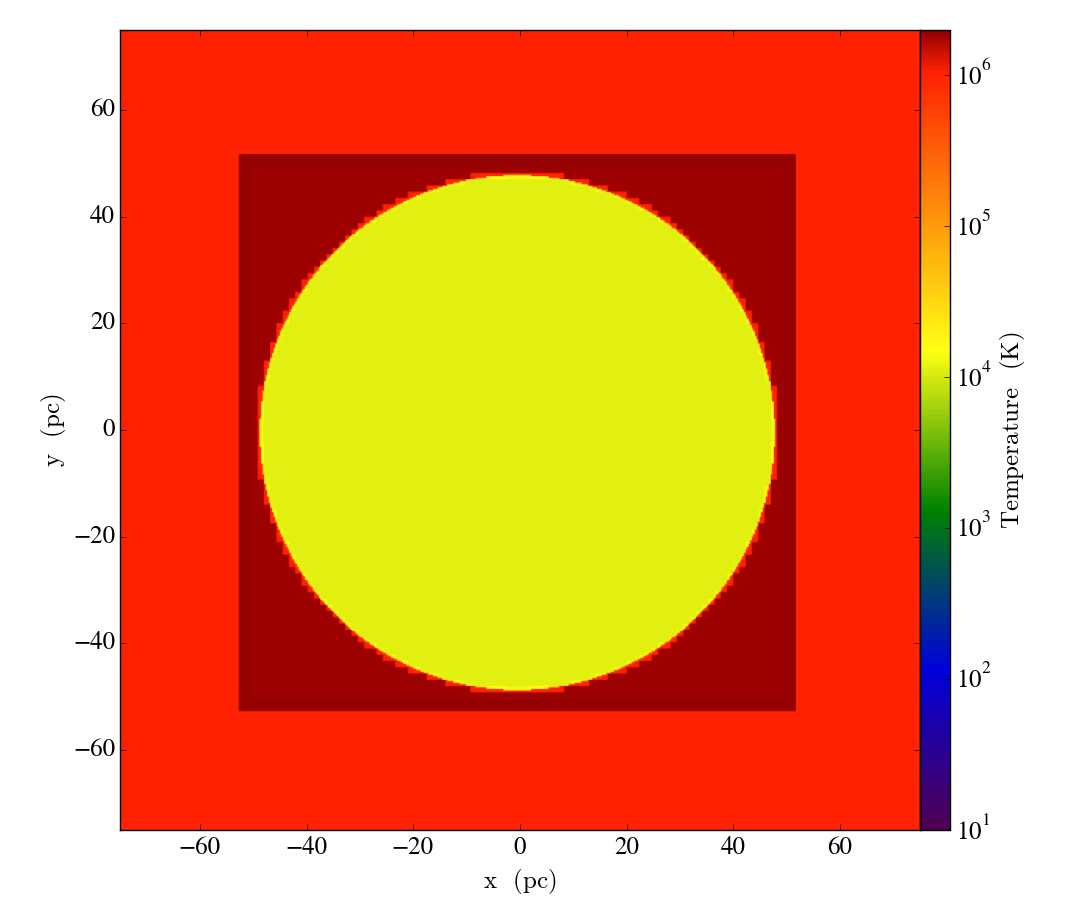
\includegraphics[width=6cm]{Images/Initial_temperature}
\end{center}
\caption{\label{fig:initial_setup} Slices showing the number density and temperature 
for the initial conditions used in this paper. }
\end{figure}

%% ----------------------------------------------------------------
% 
\section{Results}
\label{sec:results}

We now carry out a set of simulations exploring the evolution of this cloud under a variety of conditions, with a particular emphasis on the impact of metallicity on their evolution.  We begin, for simplicity, with models without any radiative background.

\subsection{No Heating Runs}

\subsubsection{$Z=10^{-3}Z_\odot$}

\begin{figure}
\begin{center}
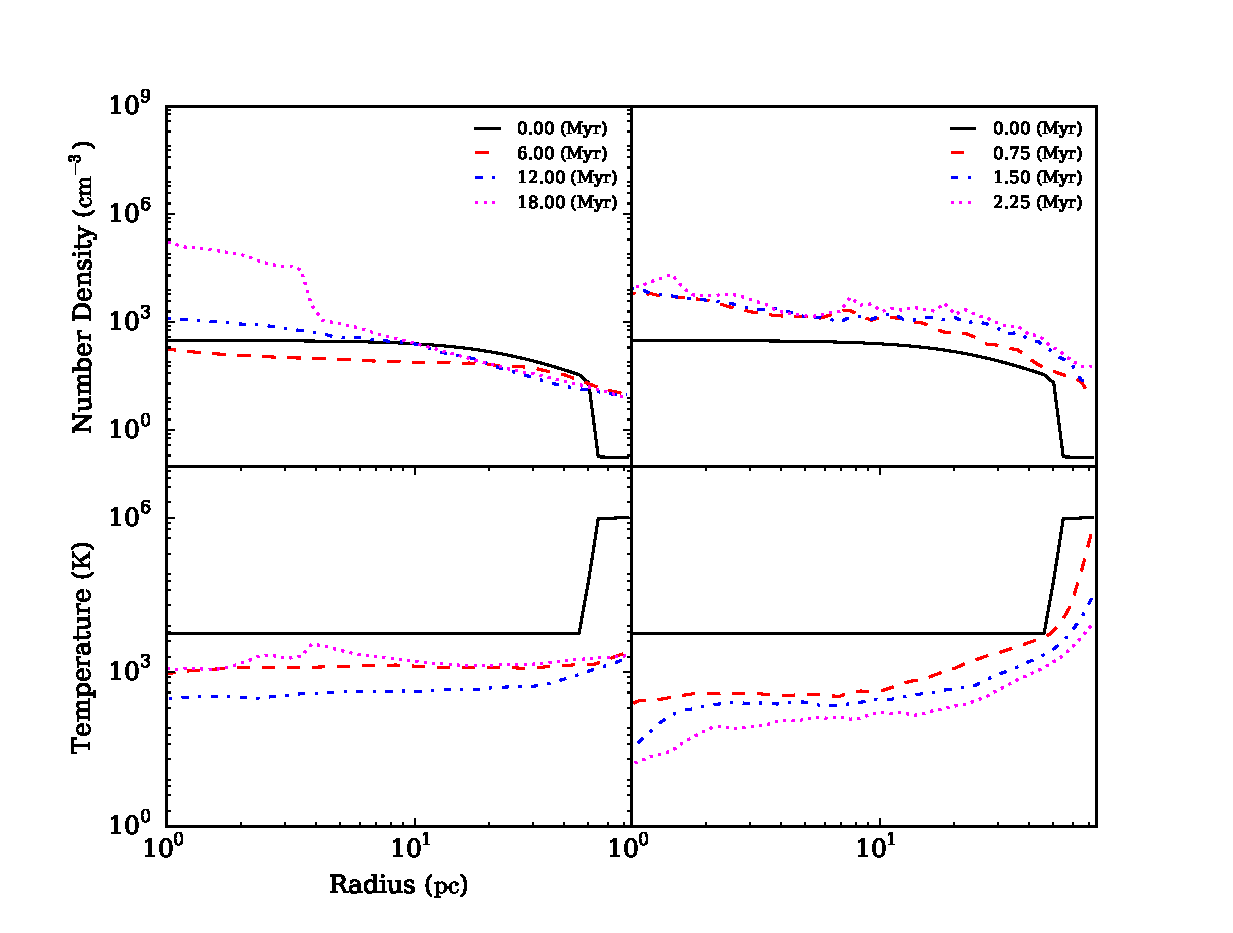
\includegraphics[width=9.5cm]{Images/profile_panel}
\end{center}
\caption{\label{fig:profiles} Cell mass weighted profiles for 
density (top panel) and temperature (bottom panel) as a function of radius at various 
output times, as shown, for runs with cooling, turbulence, and metallicity of $Z=10^{-3}Z_\odot$
(left column) and $Z=10^{-3}Z_\odot$ (right column).}
\end{figure}

We start with a low metallicity gas -- adopting $Z=10^{-3}Z_\odot$ puts us well into the regime
where the gas cooling time is longer than the gravitational collapse time (see the previous section).
In the left panels of Figure~\ref{fig:profiles}, we show density and temperature profiles at a range of times during
the collapse, stopping when high densities are reached and we can no longer accurately follow the evolution
(the Jeans length criteria cannot be met even at our highest allowed refinement level).  
The cloud, which is initially stable (i.e. in pressure equilibrium), starts to evolve due to both the added
turbulence and to gravity plus cooling. The free fall time of the cloud is $t_{ff}\approx 3$ Myr.
However, the slow cooling time delays the immediate large scale collapse.
This can be seen by the flat density profiles at times earlier than about 15 Myr. 
In fact, the cloud initially expands due to the added turbulence. The outer rim
of the cloud moves outward, initially decreasing the density in the center.
The expansion lasts for approximately 10 Myr, and during this time the temperature drops moderately
(by about a factor of 2), mostly due to the expansion.  By 18 Myr, the gravitational
collapse sets in and a dense central core forms.   The bottom left hand panel of Figure~\ref{fig:profiles}
shows the temperature profiles, with the temperature rising mildly during the recollapse, but
not heating above about 1000 K due to radiative cooling.

More detail of this collapse can be seen in Figure~\ref{fig:number_density_panel}, which shows the slices of density (left set of 6 panels) and temperature (right set of 6 panels) for this low metallicity run on the left side of each set of panels.  We select the same times as in Figure~\ref{fig:profiles} (6, 12 and 18 Myr after the initial time).  Clearly the the turbulence drives substantial fluctuations in the density (and temperature), but the cloud does not fragment, undergoing global collapse.   As expected from the one zone model, the cloud cannot efficiently cool before global gravitational collapse sets in.

\begin{figure*}
\begin{center}
\hspace{-1.2cm}
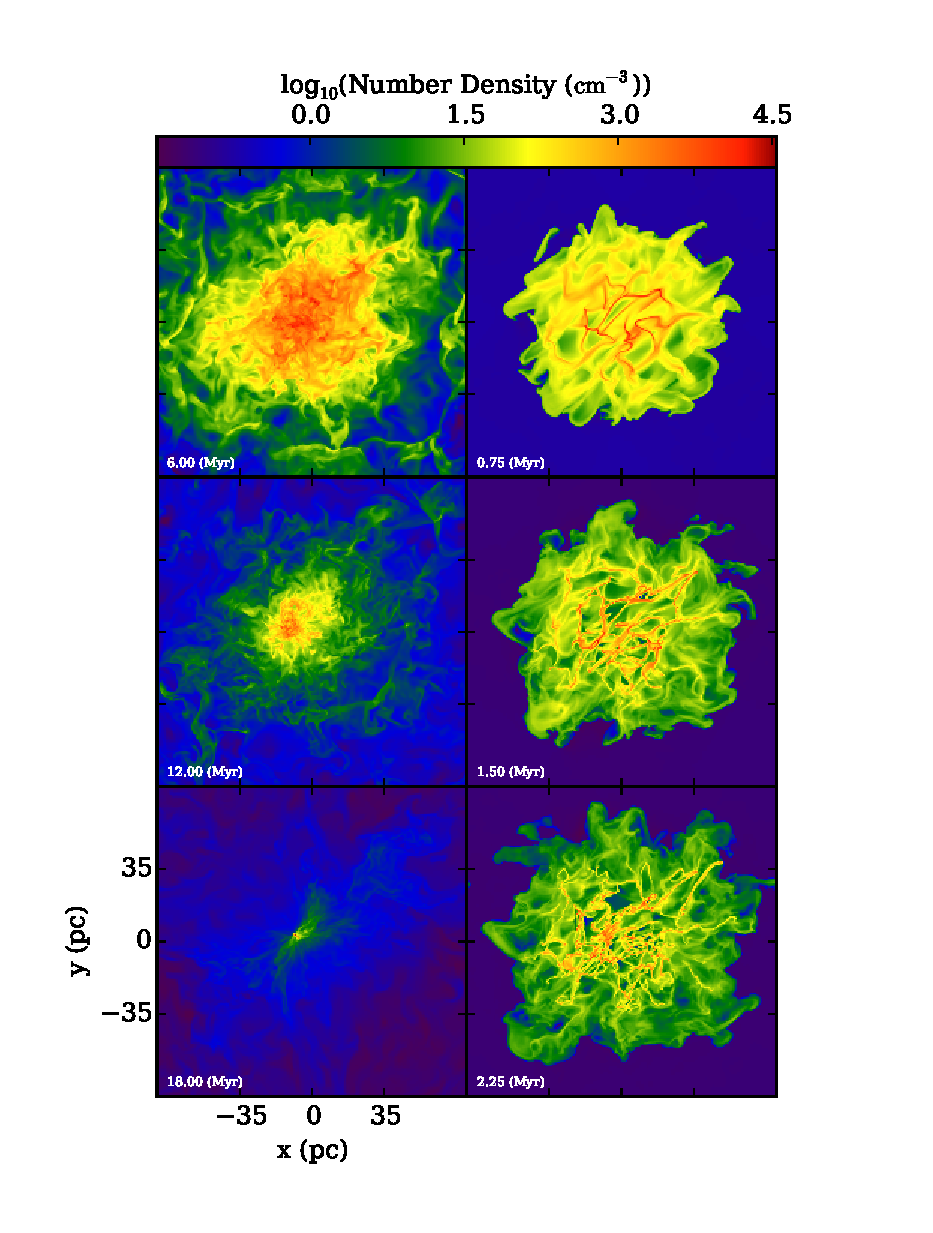
\includegraphics[width=10.3cm]{Images/slice_number_density_panel} \hspace{-2cm}
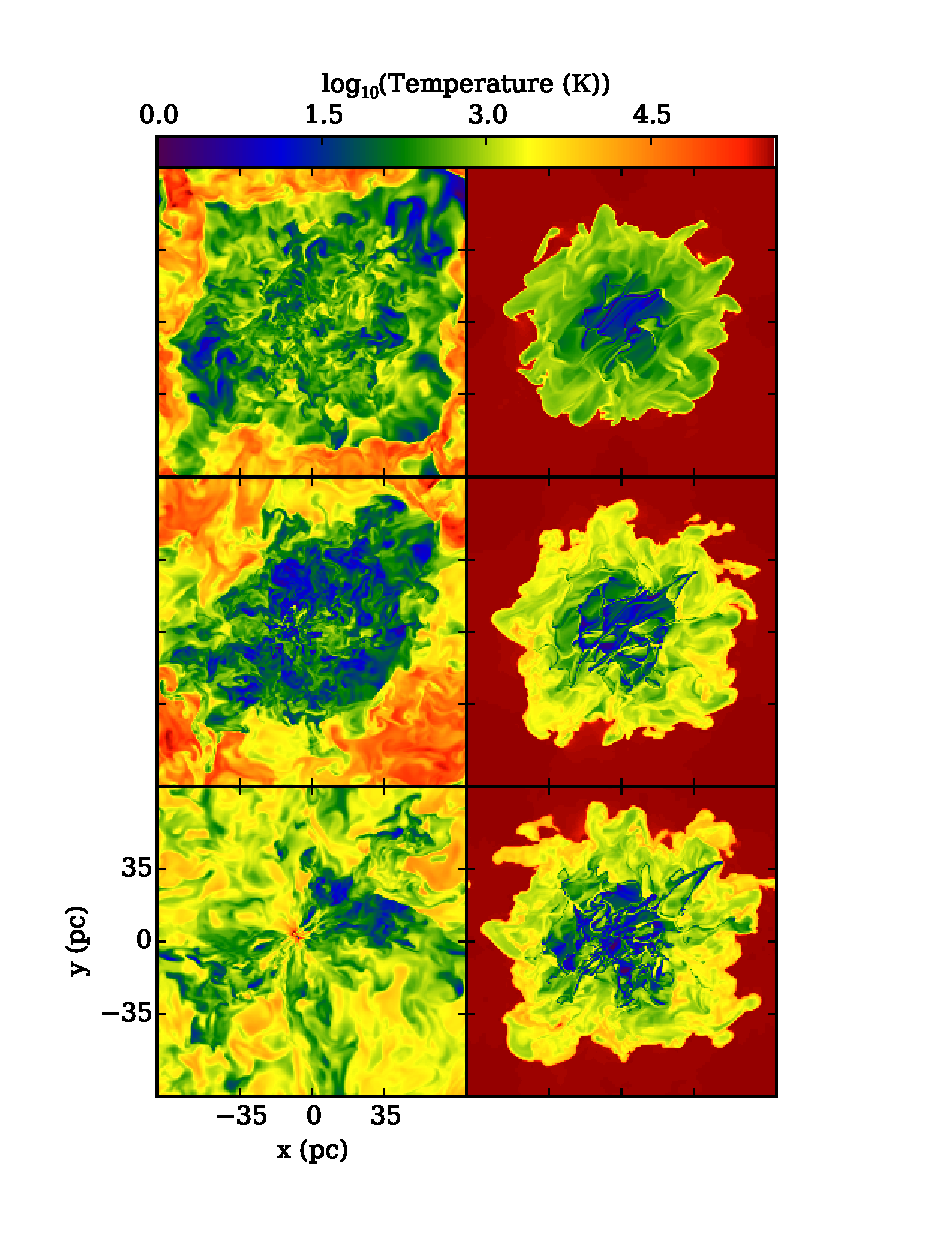
\includegraphics[width=10.3cm]{Images/temperature_panel}
\end{center}
\caption{\label{fig:number_density_panel} Density (left) and temperature (right) slices of the evolution of the sphere without radiative heating.  Time evolution is from top to bottom and in each set of 6 panels, the left side is for the low metallicity ($Z=10^{-3}Z_\odot$) run and the right-side side is for the higher (($Z=10^{-3}Z_\odot$) run.  The times are the same times as shown in the profiles in Figure~\ref{fig:profiles}.  }
\end{figure*}

%\begin{figure}
%\begin{center}
%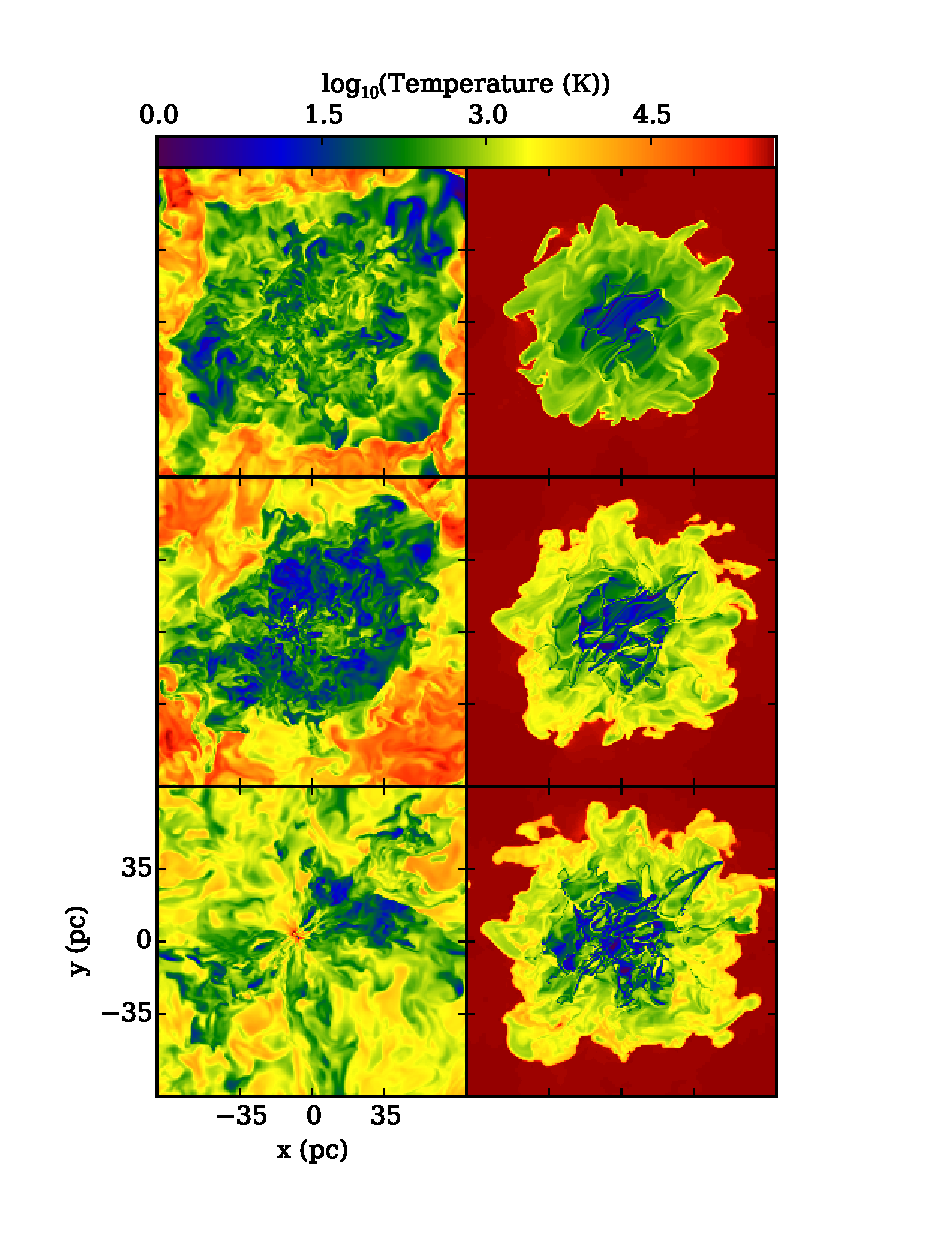
\includegraphics[width=10.5cm]{Images/temperature_panel}
%\end{center}
%\caption{\label{fig:temperature_panel} Temperature slices corresponding
%to Figure~\ref{fig:profiles}.}
%\end{figure}

\subsubsection{$Z=10^{-2}Z_\odot$}

We repeat the previous run except we increase the metallicity to $Z=10^{-2}Z_\odot$.  The profiles are shown
in the right-hand side of Figure~\ref{fig:profiles} and the density/temperature slices on the right-hand side of the panels in Figure~\ref{fig:number_density_panel}.  In this case the evolution is very different.
The gas can now cool efficiently, as evident particularly in the temperature profiles.   The center
of the gas cloud, up to radii of $\approx 10$ pc, has cooled to $\approx 200$ K in less than a million years. The added effect of the turbulence
allows the cold gas to condense into dense pockets.  This is seen clearly in the density and temperature slices, which show the formation of many dense, self-gravitating clumps.  
Hence, we see again that our numerical runs agree with our simple one zone models. Moreover, we find that there is a critical metallicity
between $10^{-3}-10^{-2}Z_\odot$ that separates the evolution of gas cloud into either global gravitational collapse or local fragmentation. 

Note that the times shown in the profiles and slices differ between the two runs because we stop the calculation in both cases when dense gas clouds form and we are no longer able to follow the evolution even with our AMR run.  In each run, at this point, star formation would rapidly occur and so we stop the calculation.


\subsection{Heating Runs}

\begin{figure}
\begin{center}
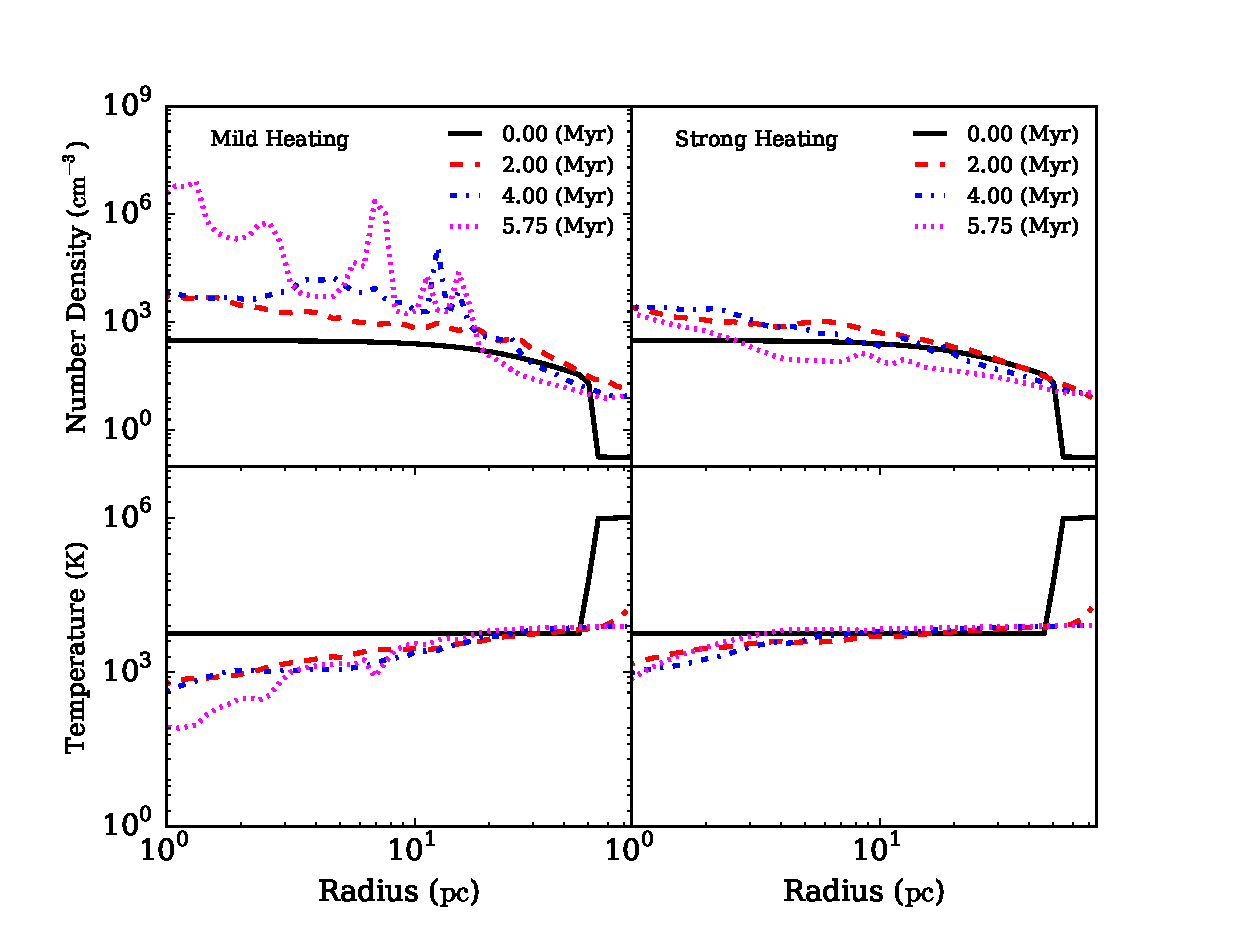
\includegraphics[width=9.5cm]{Images/profile_heating}
\end{center}
\caption{\label{fig:profiles_heating} Cell mass weighted profiles for 
density (top panel) and temperature (bottom panel) as a function of radius at various 
output times, as shown, for runs with cooling, turbulence, and metallicity of $Z=10^{-3}Z_\odot$
(left column) and $Z=10^{-3}Z_\odot$ (right column).}
\end{figure}

\begin{figure}
\begin{center}
\mbox{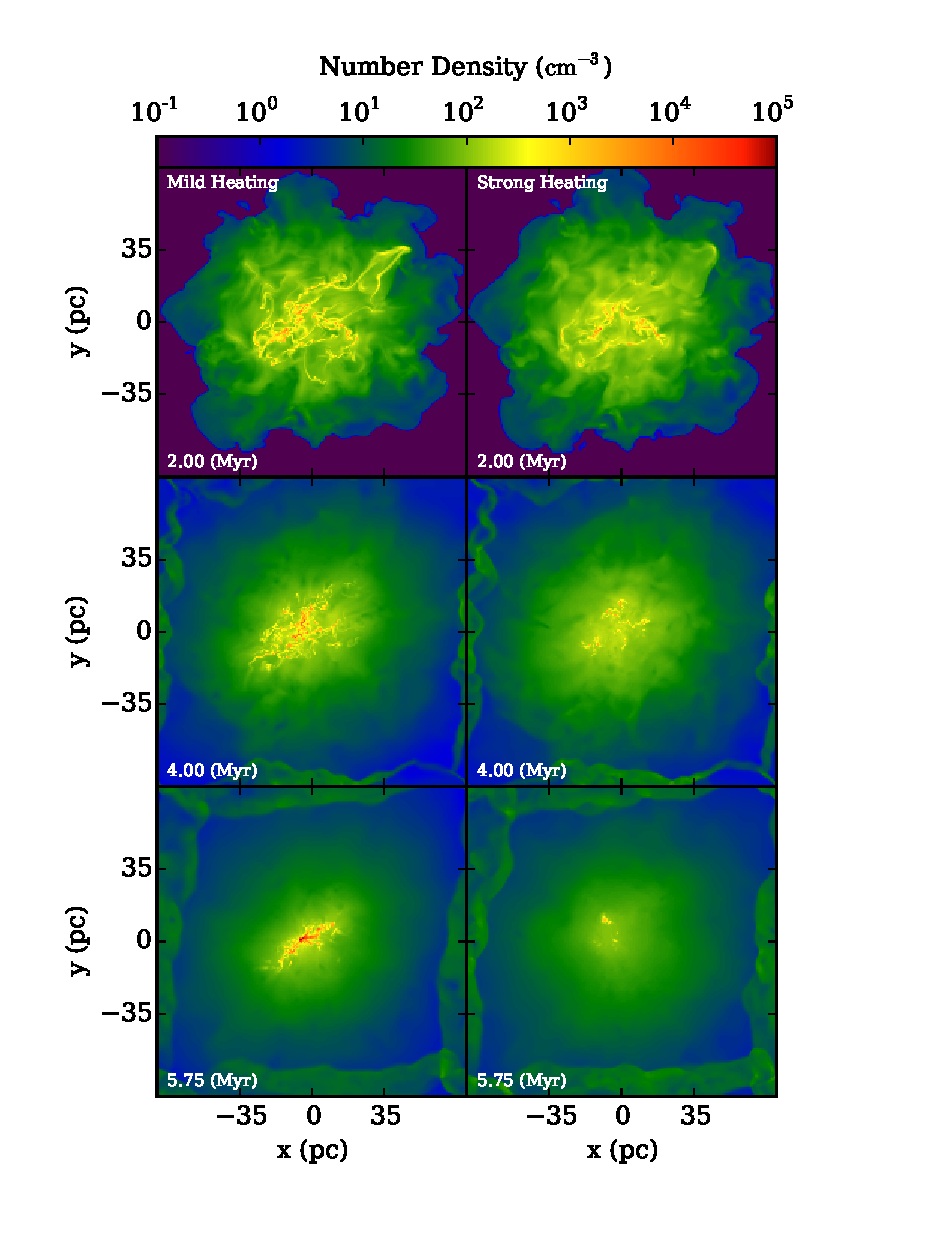
\includegraphics[width=8.5cm]{Images/density_heating_panel}}
\end{center}
\caption{\label{fig:density_heating} The ratio of cooling time to dynamical time for gas with a range of density, temperature and metallicity values, as labelled.  This plot is similar to Figure~\ref{fig:cooling_to_freefall}, except that we include a radiative heating source as specified in \citet{Haardt2012}, at $z=$0.}
\end{figure}

\begin{figure*}
\begin{center}
\hspace{-1.2cm}
\includegraphics[width=9.0cm]{Images/phase_panel} \hspace{-1cm}
\includegraphics[width=9.0cm]{Images/pressure_phase_panel}
\end{center}
\caption{\label{fig:phase_panels} Density (left) and temperature (right) slices of the evolution of the sphere without radiative heating.  Time evolution is from top to bottom and in each set of 6 panels, the left side is for the low metallicity ($Z=10^{-3}Z_\odot$) run and the right-side side is for the higher (($Z=10^{-3}Z_\odot$) run.  The times are the same times as shown in the profiles in Figure~\ref{fig:profiles}.  }
\end{figure*}

%% ----------------------------------------------------------------
% 
\section{Discussion}
\label{sec:discussion}
\subsection{Analytic Model}
\subsection{Implications}
\subsection{Caveats}

%% ----------------------------------------------------------------
% 
\section{Summary}

%% ----------------------------------------------------------------
% 
\section*{Acknowledgments}
\bibliography{mn-jour,gc_paper}
%
%\label{lastpage}
\end{document}
